%Dave's handout 1.7 intro 2nd derivatives
%Dave's handout 2.2 2nd derivative rule
\vspace{-0.25 in}
\begin{framed}
\subsection*{Objectives}
\begin{itemize}
    \item Be able to use the \textbf{basic} derivative rule of the Natural Exponential Function in conjunction with the other rules (ex. product rule, quotient rule).
    \item Be able to use the \textbf{general} derivative rule of the Natural Exponential Function in conjunction with the other rules.
    \item Understand the interpretation and use of the derivative in the model for exponential growth or decay. 
\end{itemize}

%%%Reading Assignment%%%
\subsection*{Suggested Reading:}
\begin{itemize}
\item \cite{Calaway}\footnotemark[1]
   \begin{itemize}
        \item \emph{Section 2.3 Power and Sum Rules for Derivatives}
        \begin{itemize}
            \item Derivative Rule for Exponential Functions 
            \item Example 7
        \end{itemize}
    \end{itemize}
    \begin{itemize}
        \item \emph{Section 2.4 Chain Rule}
        \begin{itemize}
            \item Example 4 and Example 8.
        \end{itemize}
    \end{itemize}

\item \cite{openstax}\footnotemark[2]\textsuperscript{,}\footnotemark[3]
    \begin{itemize}
        \item \emph{Section 3.9 Derivative of the Exponential Function}
       
    \end{itemize}

\end{itemize}
%\subsection*{Supplemental Materials:}
%%%Key Terms%%%
\subsection*{Key Terms and Concepts:} 

\begin{multicols}{2}
\begin{itemize}
    \item Exponential functions, base $e$.
    \item Differentiation of exponential functions
    \item Model for Exponential Growth or Decay
    
\end{itemize}
\end{multicols}
\end{framed}
\footnotetext[1]{Available free to download from \url{http://www.opentextbookstore.com/details.php?id=14} .}
\footnotetext[2]{Available free to download from \url{https://openstax.org/details/books/calculus-volume-1} .}
\footnotetext[3]{Disregard any examples with trigonometry.}
\newpage
%%%%%%%%%%START LESSON CONTENT%%%%%%%%%%%%%
%\noindent\makebox[\linewidth]{\rule{\textwidth}{0.8pt}}
\Opensolutionfile{ans}[ans13]
\Opensolutionfile{ansL}[ansL13]
%%%%%%%%%%%%%%%%Start First Topic%%%%%%%%%%%%%%%%%%%%%%%%%%%%%

\noindent Section 6.1 on \href{https://openstax.org/books/college-algebra/pages/6-1-exponential-functions}{College Algebra from Openstax}, the website including collection of open-source online textbooks provides a good review of exponential functions. Since calculus studies continuous change, we will almost always use the $e$-based form of exponential equations in this course.   Therefore, you should read and focus on exponential functions with the base being the mathematical constant denoted by \emph{Euler's Number}: $e$, where $e\approx 2.71828…$. 

\begin{tcolorbox}[title={Review: The Natural Exponential Function}]

\begin{multicols}{2}
The exponential function 

$$f(x) = e^x$$

with base $e$ is so prevalent in the sciences that it is often referred to as \textit{the} exponential function or the natural exponential function.

$e \approx 2.718281828459045.....$

\textit{The number is irrational.}

\columnbreak

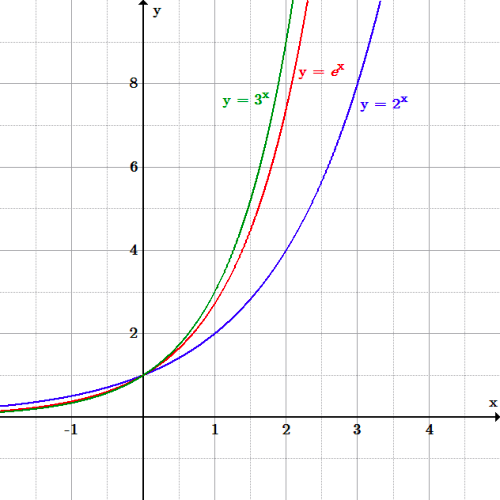
\includegraphics[scale=0.3]{images/expoFun/exponentialGraphs.png}

\end{multicols}

\end{tcolorbox}
%%%%%%%%%%%%%%%%%%%%%%%%%%%%%%%%%%%%%%%%%%%%%%%%%%%%%%%%%%%%%%%%%%%%%
\subsection*{Basic Derivative Rule of the Natural Exponential Function}
\begin{tcolorbox}[title={Derivative of the Natural Exponential Function: Basic Rule}]
Let $f(x)=e^x$ be the natural exponential function. Then
\begin{equation}\label{eq:expDerv}
    f'(x)=e^x
\end{equation}
\end{tcolorbox}
\noindent We can use the rule in equation \ref{eq:expDerv}, in conjunction with the rules we have already been given, to find derivatives of functions that include the term $ke^x$, where $k$ is a constant. 

%%%%%%%%%%%%%%%%%%%%%%%Example from Dave' handout 4.1-4.3 Exponential Functions%%%%%%%%%%%%%%%%%%%%
\begin{example}
Given $g(x)=x^2\cdot e^x$, answer the following questions:
\renewcommand{\labelenumi}{\textbf{(\alph{enumi})}}
\begin{enumerate}[leftmargin=*]
\item Find $g'(x)$.\vspace*{\stretch{1}}
\item Find all values of $x$ for which the slope of the tangent line to the graph of $g(x)$ equals 0.\vspace*{\stretch{1}}
\newpage
\item Find the intervals in which $g(x)$ is increasing and the intervals in which $g(x)$ is decreasing.\vspace*{\stretch{1}}
\end{enumerate}
    %%short answer
    \begin{sol}
    \onehalfspacing{
    \begin{enumInline1}
    \item $g'(x)=xe^x(x+2)$
    \item $x=-2,0$
    \item Increasing on $(-\infty,-2)\cup (0,\infty)$; decreasing on $(-2,0)$
    \end{enumInline1} }
    \end{sol}
    %%solution
    \begin{solL}
    Complete solution here.....
    
    \end{solL}
    
\end{example}

%%%%%%%%%%%%%%%%%%%%%%%Example from Dave' handout 4.1-4.3 Exponential Functions%%%%%%%%%%%%%%%%%%%%
\begin{example}
Given $g(x)=\displaystyle\frac{2x+1}{e^x}$, answer the following questions:
\renewcommand{\labelenumi}{\textbf{(\alph{enumi})}}
\begin{enumerate}[leftmargin=*]
\item Find $g'(x)$.\vspace*{\stretch{1}}
\item Find all values of $x$ for which the slope of the tangent line to the graph of $g(x)$ equals 0.\vspace*{\stretch{1}}

\item Find the intervals in which $g(x)$ is increasing and the intervals in which $g(x)$ is decreasing.\vspace*{\stretch{1}}
\end{enumerate}
    %%short answer
    \begin{sol}
    \onehalfspacing{
    \begin{enumInline1}
    \item $g'(x)=\displaystyle\frac{-2x+1}{e^x}$
    \item $x=\frac{1}{2}$
    \item Increasing on $\left(-\infty,\frac{1}{2}\right)$; decreasing on $\left(\frac{1}{2},\infty\right)$
    \end{enumInline1} }
    \end{sol}
    %%solution
    \begin{solL}
    Complete solution here.....
    
    \end{solL}
    
\end{example}
\newpage
%%%%%%%%%%%%%%%%%%%%%%%Example from Dave' handout 4.1-4.3 Exponential Functions%%%%%%%%%%%%%%%%%%%%
\begin{example}
Find the slope of the tangent line to the graph of  $g(x)=\displaystyle\frac{e^x}{x+e^x }$ at the point $(0, 1)$.\vspace*{\stretch{1}}
\end{example}
%%short answer
    \begin{sol}
    slope $=-1$
    \end{sol}
    %%solution
    \begin{solL}
    Complete solution here.....
    
    \end{solL}
%%%%%%%%%%%%%%%%%%%%%%%Example from Dave' handout 4.1-4.3 Exponential Functions%%%%%%%%%%%%%%%%%%%%
\begin{example}
Given $g(x)=e^x(1-e^x)^2$, answer the following questions:
\renewcommand{\labelenumi}{\textbf{(\alph{enumi})}}
\begin{enumerate}[leftmargin=*]
\item Find $g'(x)$.\vspace*{\stretch{1}}
\item Find all values of $x$ for which the slope of the tangent line to the graph of $g(x)$ equals 0.\vspace*{\stretch{1}}
\end{enumerate}
    %%short answer
    \begin{sol}
    \onehalfspacing{
    \begin{enumInline1}
    \item $x=0$
    \item $x=ln\left(\frac{1}{3}\right)$

    \end{enumInline1} }
    \end{sol}
    %%solution
    \begin{solL}
    Complete solution here.....
    
    \end{solL}
    
\end{example}
\newpage
%%%%%%%%%%%%%%%%%%%%%%%%%%%%%%%%%%%%%%%%%%%%%%%%%%%%%%%%%%%%%%%%%%%%%
\subsection*{General Derivative Rule of the Natural Exponential Function}
\noindent Section \ref{GenPower} uses the Chain Rule to provide a more general rule for differentiating exponential functions, a rule that is needed when the exponent on the base $e$ is not simply $x$, but rather a function of $x$.
\begin{tcolorbox}[title={Derivative of the Natural Exponential Function: General Rule}]
If $f(x)=e^{g(x)}$, then
\begin{equation}\label{eq:GenexpDerv}
    f'(x)=e^{g(x)}\cdot g'(x)
\end{equation}
\end{tcolorbox}
%%%%%%%%%%%%%%%%%%%%%%%Example from Dave' handout 4.1-4.3 Exponential Functions%%%%%%%%%%%%%%%%%%%%
\begin{example}
Given $g(x)=x\cdot e^{x^2}$, answer the following questions:
\renewcommand{\labelenumi}{\textbf{(\alph{enumi})}}
\begin{enumerate}[leftmargin=*]
\item Find $g'(x)$.\vspace*{\stretch{1}}
\item Find all values of $x$ for which the slope of the tangent line to the graph of $g(x)$ equals 0.\vspace*{\stretch{1}}
\item Find all relative maximum and relative minimum points.\vspace*{\stretch{1}}
\end{enumerate}
    %%short answer
    \begin{sol}
    \onehalfspacing{
    \begin{enumInline1}
    \item $g'(x)=e^{x^2}(2x^2+1)$
    \item None
    \item None
    \end{enumInline1} }
    \end{sol}
    %%solution
    \begin{solL}
    Complete solution here.....
    
    \end{solL}
    
\end{example}
\newpage
%%%%%%%%%%%%%%%%%%%%%%%Example from Dave' handout 4.1-4.3 Exponential Functions%%%%%%%%%%%%%%%%%%%%
\begin{example}
Given $g(x)=\displaystyle\frac{e^{2x+1}}{x^2}$, answer the following questions:
\renewcommand{\labelenumi}{\textbf{(\alph{enumi})}}
\begin{enumerate}[leftmargin=*]
\item Find $g'(x)$.\vspace*{\stretch{1}}
\item Find all values of $x$ for which the slope of the tangent line to the graph of $g(x)$ equals 0.\vspace*{\stretch{1}}

\item Find the intervals in which $g(x)$ is increasing and the intervals in which $g(x)$ is decreasing.\vspace*{\stretch{1}}
\end{enumerate}
    %%short answer
    \begin{sol}
    \onehalfspacing{
    \begin{enumInline1}
    \item $g'(x)=\displaystyle\frac{2e^{2x+1}\cdot (x-1)}{x^3}$
    \item $x=1$
    \item Increasing on $(-\infty,0)\cup (1,\infty)$; decreasing on $(0,1)$
    \end{enumInline1} }
    \end{sol}
    %%solution
    \begin{solL}
    Complete solution here.....
    
    \end{solL}
    
\end{example}
\newpage
%%%%%%%%%%%%%%%%%%%%%%%%%%%%%%%%%%%%%%%%%%%%%%%%%%%%%%%%%%%%%%%%%%%%%
\subsection*{Applying the Natural Exponential Function}
%%%%%%%%%%%%%%%%%Pata's MATH 1050 workbook: Lesson 17 Exponential Functions%%%%%%%%%%%%%%%%%%%
%%%%%%%%%%%%%%%%%%%%%%%%%%%%%%%%%%%%%%%%%%%%%%%%%%%%%%%%%%%%%%%%
\begin{tcolorbox}[title=Review: Continuous Compound Interest Formula]
$$A = Pe^{rt}$$

$A = $ amount after $t$ years

$P=$ principal

$r=$ annual interest rate (expressed as a decimal)

$t=$ number of years
\end{tcolorbox}
%%%%%%%%%%%%%%%%%%%%%%%%%%%%%%%%%%%%%%%%%%%%%%%%%%%%%%%%%%%%%%%%%%%
%%%%%%%%%%%%%%%%%%%%%%%Example from OpenStax Example 3.76%%%%%%%%%%%%%%%%%%%%
\begin{example}
Suppose you invest \$10,000 in an account that pays \emph{continuously compounded interest} at an annual rate of 5\%.
\renewcommand{\labelenumi}{\textbf{(\alph{enumi})}}
\begin{enumerate}[leftmargin=*]
\item Determine the appropriate function $A(t)$.\vspace*{\stretch{1}}
\item How much money will be in the account at time $t=5$ years from the present?\vspace*{\stretch{1}}
\item Find $A'(5)$. Interpret the result. \vspace*{\stretch{1}}
\newpage

\end{enumerate}
    %%short answer
    \begin{sol}
    \onehalfspacing{
    \begin{enumInline1}
    \item $A(t)=10,000e^{0.05t}$
    \item $A(5)\approx 12840.25$ dollars.
    \item $A'(t)=500e^{0.05t}$;$A'(5)\approx 642.01$;  At the $5^{th}$ year, your investment is increasing at the rate of (around) 642.01 dollars per year.
    \end{enumInline1} }
    
    \end{sol}
    %%solution
    \begin{solL}
    Complete solution here.....
    
    \end{solL}
    
\end{example}
\begin{tcolorbox}[title={Review: Model for Exponential Growth or Decay}]

For $k >0$,
\textbf{Exponential Growth:} $A(t) = A_0e^{kt}$,

\textbf{Exponential Decay:} $A(t) = A_0 e^{-kt}$

where,

$A(t)$ = the amount at time $t$

$A_0 = A(0)$, the initial amount (the amount at $t=0$)

$k = $relative rate of growth or decay.

$t=$ time

\textit{\textbf{Continuously Compound Interest} is an example for Exponential Growth.}

\end{tcolorbox}

%%%%%%%%%%%%%%%%%%%%%%%Example from OpenStax Example 3.76%%%%%%%%%%%%%%%%%%%%
\begin{example}
A colony of mosquitoes has an initial population of 1000. After $t$ days, the population is given by $A(t)=1000e^{0.3t}$. 
\renewcommand{\labelenumi}{\textbf{(\alph{enumi})}}
\begin{enumerate}[leftmargin=*]
\item The \textbf{relative rate of growth} or the \textbf{growth factor} is the ratio of the rate of change of the population, $A'(t)$, to the population , $A'(t)$, to the population, $A(t)$. Show that the \textbf{relative rate of growth} of  mosquitoes population is constant.\vspace*{\stretch{1}}
\item What is the \textbf{rate of change} of mosquitoes population after 4 days?. Interpret the result.\vspace*{\stretch{1}}
\item What is the \textbf{growth factor} of mosquitoes population after 4 days? Interpret the result. \vspace*{\stretch{1}}
\newpage

\end{enumerate}
    %%short answer
    \begin{sol}
    \onehalfspacing{
    \begin{enumInline1}
    \item $A'(t)=300e^{0.3t}\Longrightarrow \displaystyle\frac{A'(t)}{A(t)}=\displaystyle\frac{300e^{0.3t}}{A(t)}=\displaystyle\frac{300e^{0.3t}}{1000e^{0.3t}}=0.3$
    \item After 4 days, the mosquitoes population is increasing at the rate of $A'(4)\approx 996$ mosquitoes per day.
    \item For each day, the mosquitoes population has multiplied itself by 103\% (by a factor of 3).
    \end{enumInline1} }
    
    \end{sol}
    %%solution
    \begin{solL}
    Complete solution here.....
    
    \end{solL}
    
\end{example}

%%%%%%%%%%%%End Examples%%%%%%%%%%%%%%%%%%




%%%%%%%%%%%%%%%End Lesson%%%%%%%%%%%%%%%%%%
\Closesolutionfile{ans}
\Closesolutionfile{ansL}

%%%Short Answers to Examples%%%
\newpage
%\vspace*{\fill}

\subsection*{Short Answers to Examples}
%\vspace{-0.25cm}
%\begin{multicols}{2}
\input{ans13}
%\end{multicols}


